\documentclass[lang=cn,10pt]{AbsBook}
\usepackage[a4paper,
			left=3.17cm,
			right=3.17cm,
			top=2.54cm,
			bottom=2.54cm]{geometry}
\tcbuselibrary{listings}
\usepackage{forloop}
\usepackage{datetime2}
\usepackage{datetime2-calc}

\title{Linux/\LaTeX{}使用技巧}
%\subtitle{Abs\LaTeX{} 经典之作}

\author{陈潇}
\version{0.0.1}
\Publisher{XX出版社}
%\BookSeries{计算机科学系列丛书}

\BookIntroduction{
现在的AbsBook模板是将ElegantBook与ChenLaTeXBook两个模板进行组合得到的新模板,封面封底选了ChenLaTeXBook的设计,其余部分基本都是ElegantBook的设计,参考文献的生成方式改成了用\hologo{BibTeX}来生成,在书的末尾部分增加了索引。
}
\AuthorIntroduction{这里是一些测试文字。}

\Innovation{著}					   %著、编、编著
%------------扉页反面-----------
\PublisherAddress{北京}			   %出版社地址
\Price{5}							%价格

\Word{500}							%字数, 单位: 千
\CIP{555555}						%CIP数据核字号
\isbn{978-7-03-071008-6}

\RomanI{2135}						%
\RomanIII{测试---使用---abcd}
\RomanIV{I399}						%

\Website{https://2tap.cf}			%网站
\Prints{001-1000000}				%印数

\setcounter{tocdepth}{3}
% 本文档命令
\usepackage{array}
\newcommand{\ccr}[1]{\makecell{{\color{#1}\rule{1cm}{1cm}}}}

% \definecolor{customcolor}{RGB}{32,178,170}
% \colorlet{coverlinecolor}{customcolor}

\makeindex
\begin{document}

\maketitle
\makeflypage
\frontmatter

\tableofcontents

\mainmatter

\part{日常使用}

\chapter{实用软件}
\section{腾讯QQ}
\subsection{官方版本}
首先,我们先登录\href{https://im.qq.com/download/}{腾讯QQ官网},然后我们找到QQ Linux版,如下图~\ref{fig:download-qq}所示:

\begin{figure}[htbp]
	\centering
	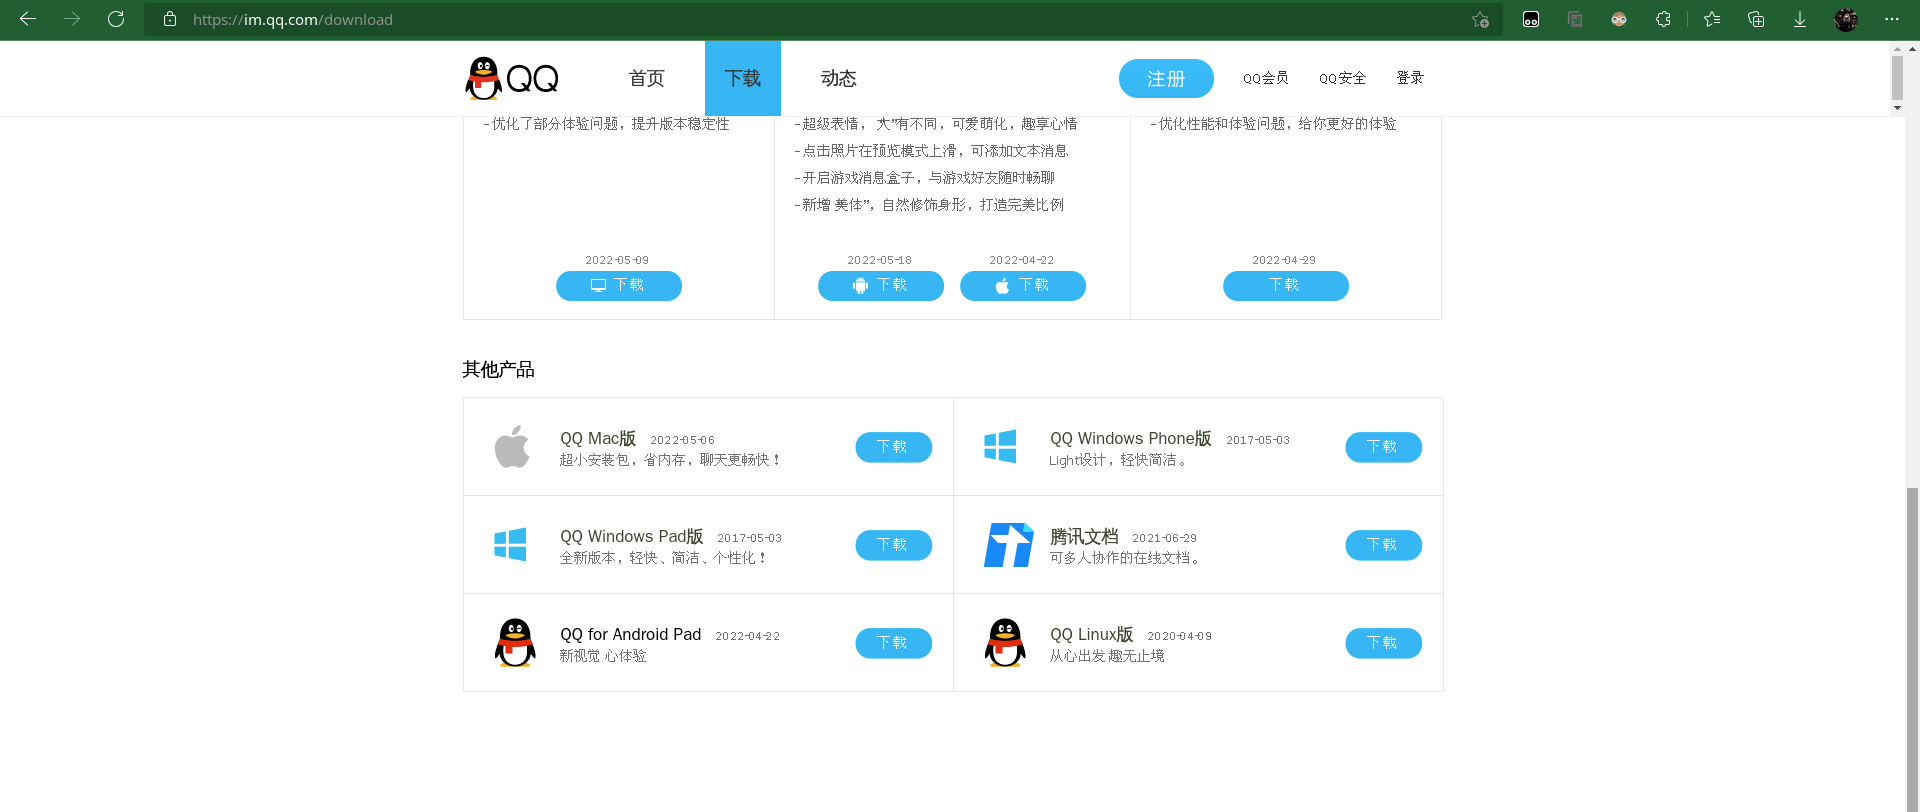
\includegraphics[width=\textwidth]{qq-download}
	\caption{QQ官网下载页}\label{fig:download-qq}
\end{figure}

如图~\ref{fig:qq-version}~选择自己合适的版本下载即可(可以使用\lstinline|uname -a|命令查看架构)
\begin{figure}[htbp]
	\centering
	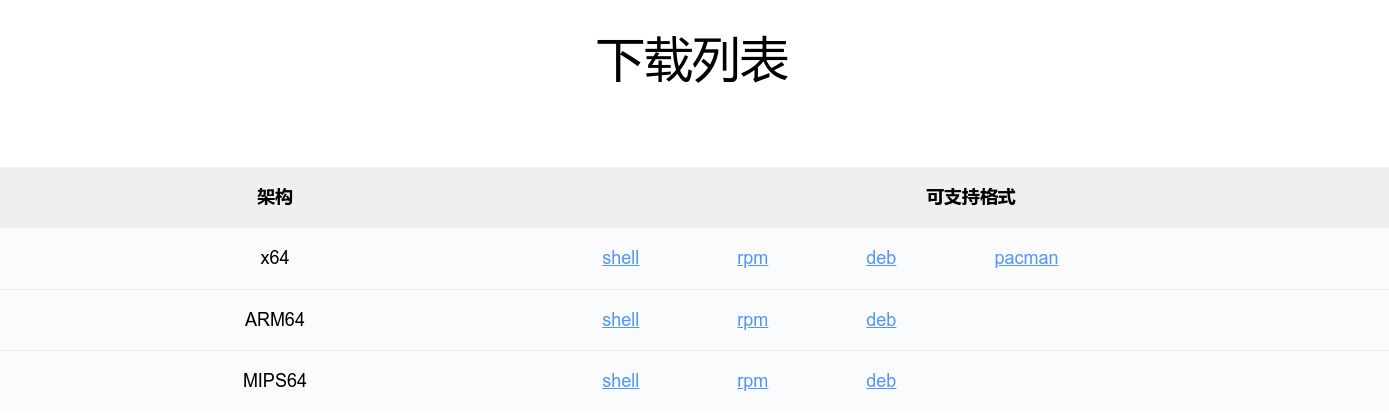
\includegraphics[width=\textwidth]{qq-version}
	\caption{QQ官网下载页}\label{fig:qq-version}
\end{figure}

下载好之后,将工作目录切换至下载的目录,使用命令
\begin{lstlisting}
sudo dpkg -i linuxqq*.deb
\end{lstlisting}
安装。安装好之后,在终端使用\lstinline|qq|命令或者在程序列表里就可以打开了。

若扫码后出现闪退的情况,可以尝试使用以下命令删除配置文件:
\begin{lstlisting}
sudo rm -rf ~/.config/tencent-qq/你的QQ号
\end{lstlisting}

\subsection{icalingua++}
Icalingua++ 是 Icalingua 的分支,为已经删除的 Icalingua 提供有限的更新。该项目希望为 Linux 打造一个会话前端框架,通过实现 Adapter 后端接口来适配各种聊天平台。目前已经拥有基于 oicq 以及 Icalingua 自有协议的后端。

\href{https://github.com/Icalingua-plus-plus/Icalingua-plus-plus}{GitHub}上可以找到最新版本,在release中可以找到对应GNU/Linux发行版的安装包或APPImage二进制文件,使用对应的命令安装使用即可。

\section{微信}
\subsection{Wine-Wechat}
\subsubsection{安装Wine}
在Debian11下安装Wine很简单,只需要一条命令即可
\begin{lstlisting}
$sudo apt-get install wine
\end{lstlisting}

安装好Wine之后,在终端输入\lstinline|winecfg|命令来对Wine进行设置
\begin{itemize}
	\item 在Application选项卡下,将Windows 版本设置为Windows10
	\begin{figure}[htbp]
		\centering
		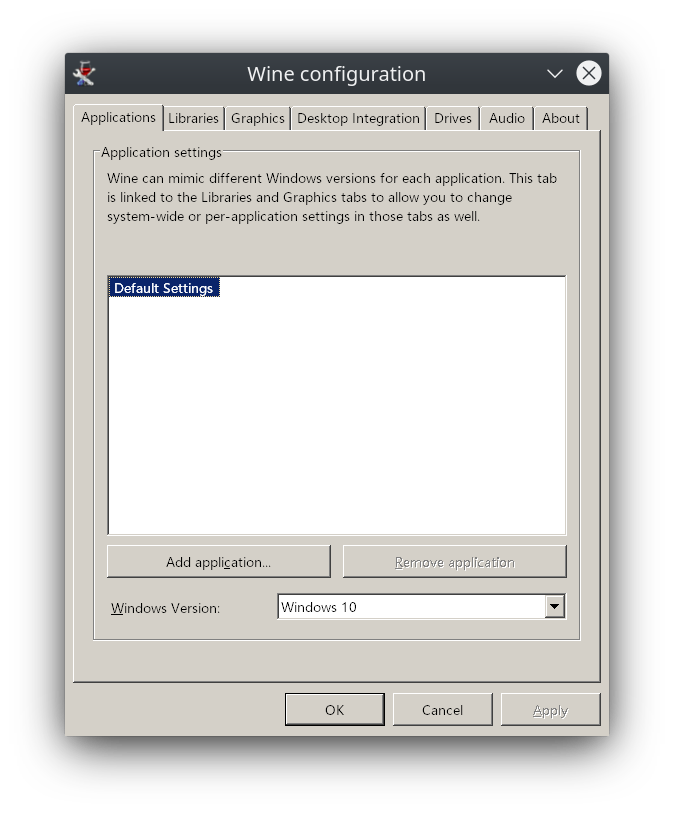
\includegraphics[height=8cm]{WindowsVersion}
		\caption{设置Windows版本}
	\end{figure}
	\item 在Graphic选项卡下,将DPI调整至120左右,较高的DPI会有一个比较好的显示效果。~图\ref{dpi}
	\begin{figure}[htbp]
		\centering
		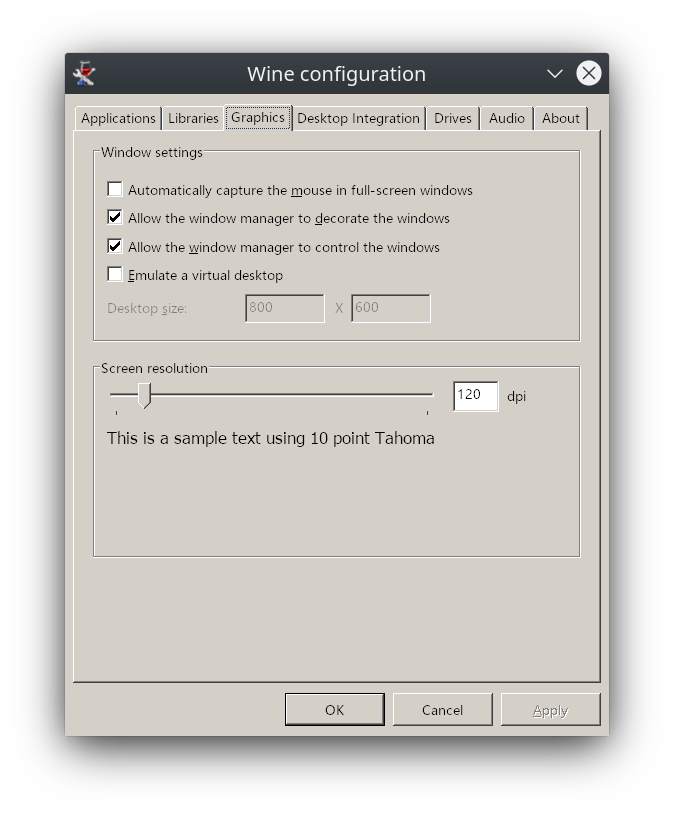
\includegraphics[height=8cm]{DPI}
		\caption{DPI设置}\label{dpi}
	\end{figure}
\end{itemize}

设置好之后,使用
\begin{lstlisting}
	wine WeChatSetup.exe
\end{lstlisting}
命令安装微信(同理,也可以使用此命令安装其他exe文件)。

安装完成之后,还需要去解决中文字体无法显示问题以及无法输入的问题。

\subsubsection{中文字体无法显示问题}
首先需要从Windows字库中获取到\lstinline|msyh.tcc|文件,拷贝到Wine的工作目录下。
\begin{lstlisting}
	cp msyh.ttc ~/.wine/drive_c/windows/Fonts
\end{lstlisting}

新建一个文本文件,保存为\verb*|font.reg|,内容如下:
\lstinputlisting{code/font.reg}

使用命令\begin{lstlisting}
	wine ~/.wine/drive_c/windows/regdit.exe font.reg
\end{lstlisting}
之后重启微信,中文就可以正常显示了。

\subsubsection{聊天框无法输入文字}
首先安装winetricks
\begin{lstlisting}
	sudo apt-get install winetricks
\end{lstlisting}
在\lstinline|~/.cache/winetricks|文件夹下,创建两个名为\lstinline|msls31|和\lstinline|win2ksp4|的文件夹,将\lstinline| InstMsiW.exe|文件放进\lstinline|msls31|目录,将\lstinline| W2KSP4_EN.EXE|文件放进\lstinline|win2ksp4|目录。

执行
\begin{lstlisting}
	winetricks riched20
\end{lstlisting}
命令,等到命令修复完成后重启微信,就可以正常使用了。


\subsection{Linux原生微信}
Linux原生的微信安装就比较简单,但原生微信是对统信UOS系统“特供”的,在安装的时候会有一个对操作系统的验证,所以需要安装一个包来把Debian系统“伪装”成国产的统信系统。用两次dpkg命令就可以安装好了。
\begin{lstlisting}
	sudo dpkg -i install-this-first.deb
	sudo dpkg -i wechat-linux-spark_2.1.2-1_amd64.deb
\end{lstlisting}
\subsection{二者对比}
其实使用起来两个都不怎么好用,Wine下的无法访问剪贴板、传输文件很麻烦;原生的实际上就是个浏览器套壳,没有时间戳、消息提示,每次登录都得扫码,用起来也很麻烦。


\part{生产开发}

\chapter{\LaTeX{}使用}

\section{实用宏包介绍}
\subsection{tcolorbox -- 漂亮的盒子}
tcolorbox宏包能制作风格多样、非常漂亮的盒子,用来写书籍或者是一些比较花哨的文档时,可以使用。
以下是一个例子:

\begin{tcolorbox}[title = tcolorbox的官方文档链接]
	\url{https://mirrors.bfsu.edu.cn/CTAN/macros/latex/contrib/tcolorbox/tcolorbox.pdf}
\end{tcolorbox}
\begin{tcolorbox}[title = tcolorbox的一些使用例子,colframe=red!50!white]
	\url{https://mirrors.sustech.edu.cn/CTAN/macros/latex/contrib/tcolorbox/tcolorbox-example.pdf}
\end{tcolorbox}

特别是用来写Linux命令终端的时候,就非常的炫酷:
\begin{tcolorbox}
	\begin{lstlisting}[language=Tex]
		\newtcblisting{commanshell}{colback=black,colupper=white,colframe=yellow!75!black,listing only, listing options={style=tcblatex,language=sh},every listing line={\textcolor{red}{\small\ttfamily\bfseries root \$> }}}
		\begin{commanshell}
			ls -al
			cd /usr/lib
		\end{commanshell}
	\end{lstlisting}
	\tcblower
	\newtcblisting{commanshell}{colback=black,colupper=white,colframe=yellow!75!black,listing only, listing options={style=tcblatex,language=sh},every listing line={\textcolor{red}{\small\ttfamily\bfseries root \$> }}}

	\begin{commanshell}
ls -al
cd /usr/lib
	\end{commanshell}
\end{tcolorbox}
这个宏包的用途还有很多,也可以用来放代码、定理、例子等等特殊环境。

\subsection{lstinline命令}
使用\lstinline$\lstinline|code|$命令来生成行内公式或者命令,会比\lstinline|\verb|命令好得多,不会突出空格。
\begin{tcolorbox}[title = 使用verb的效果,colframe=blue]
	\verb*|$mv source destination|
\end{tcolorbox}
\begin{tcolorbox}[title=使用lstinline的效果,colframe=orange!50!white]
	\lstinline|$mv source destination|
\end{tcolorbox}

\subsection{printlen -- 输出纸张大小}
在输出纸张开本大小的时候,可以在引入printlen宏包之后,使用\lstinline|\rndprintlength{\paperwidth}$\times$\rndprintlength{\paperheight}|命令,这样可以自动生成纸张大小,不用自己手动输入。
\begin{tcolorbox}[title=效果,colframe=red]
	开本:\rndprintlength{\paperwidth}$\times$\rndprintlength{\paperheight}
\end{tcolorbox}

\subsection{geometry -- 管理页面规格}
geometry宏包可以灵活地管理页面规格,常用的参数有
\begin{itemize}
	\item paper可以设置纸张大小,具体的值有a4paper, a5paper, b6paper等等常见的纸张大小
	\item paperwidth手动设置纸的宽度
	\item paperheight手动设置纸的高度
	\item landscape将纸水平放置,横向
	\item left,right,top,bottom则是设置纸张的左右上下边距
\end{itemize}
一个使用范例为:
\begin{lstlisting}[language=TeX]
	\RequirePackage[%
	a4paper,
	left=3.17cm,
	right=3.17cm,
	top=2.54cm,
	bottom=2.54cm,
	]{geometry}
\end{lstlisting}
还有一个好用的参数: twoside,使用了这个参数以后,左边距和右边距的设置会翻页自动互换,很实用。


\subsection{hologo -- 输出\TeX{}家族字体}
导入\verb|hologo|宏包,就可以用\lstinline|\hologo{}|命令输出\TeX{}家族的特殊字体,比方说\hologo{XeLaTeX}, \hologo{LaTeX2e}, \hologo{LaTeXTeX}

\subsection{makeidx -- 生成索引}
生成索引需要用到makeidx宏包,在导言区导入后:
\begin{enumerate}
	\item	在正文索引关键字的位置使用\lstinline|\index{}|命令,这个命令就类似于\lstinline|\label|命令
	\item 在想要生成的索引的地方(书的末尾)使用\lstinline|\printindex|命令
	\item 使用\hologo{XeLaTeX}编译一遍
	\item 在文档目录下打开终端,使用\lstinline|makeindex *.idx|命令(TeXstudio可以在工具栏选Tools-Index)
	\item 再到文档中使用\hologo{XeLaTeX}编译一遍即可
\end{enumerate}

\subsection{forloop -- for循环}
想在\LaTeX 中实现for循环,可以使用forloop宏包,配合上计数器(counter,可以当做int型变量来用),就可以实现类似于其他语言中的循环语句。这个宏包中只定义了两个命令:\lstinline|\forloop|和\lstinline|\forLoop|,但后者已被弃用。

\verb|\forloop|命令的语法为:
\begin{lstlisting}
\forloop[<step>]{<counter}{<initial value>}{<condition>}{<code>}
\end{lstlisting}
在此之前,先要创建一个计数器(类似于声明变量)
\begin{lstlisting}
\newcounter{<countername>}
\end{lstlisting}
下面是一个例子:
\begin{lstlisting}
\newcounter{ct} \forloop{ct}{1}{\value{ct} < 10}{\arabic{ct}}
\end{lstlisting}
输出:\newcounter{ct} \forloop{ct}{1}{\value{ct} < 10}{\arabic{ct}}

\subsection{ean13isbn -- 生成ISBN条码}
使用\lstinline|ean13isbn|这个宏包,就可以根据ISBN号打印出条码。

但是这个命令比较奇怪,是通过在命令选项中传递参数的。不过也可以在使用\lstinline|\usepackage|命令时作为选项将ISBN传入。

\lstinline|\EANisbn[SC5a,ISBN=978-80-7340-097-2]|

这样就能生成一个带ISBN文本的条码了。
\begin{center}
	\hspace{1cm}\EANisbn[SC5a,ISBN=978-80-7340-097-2]
\end{center}
而使用\lstinline|\EAN|命令,可以生成不带文本的条码。
\begin{center}
	\hspace{1cm}\EAN 978-80-7340-097-2
\end{center}

需要注意的是,使用\lstinline|center|环境无法让条码居中,要用\lstinline|\hspace{•}|和\lstinline|\vspace{•}|配合使用,让条码改变位置,或者用Tikz调整位置。

\subsection{pdfpages -- 插入PDF文件}
对于像教学设计这种复杂又的表格,可以使用Word先制作好,再导出成PDF文件,再导入进\LaTeX 文档也是一种可行的方法。缺点是可能会有大量的空白,也没找着方法消除。

首先导入\lstinline|pdfpages|宏包
\begin{lstlisting}
\usepackage{pdfpages}
\end{lstlisting}
在想导入的位置使用
\begin{lstlisting}
\includepdf[pages=-]{XXX.pdf}
\end{lstlisting}
就可以了。

尝试过将此命令放置在\lstinline|figure|环境中,\lstinline|box|环境中,使用\lstinline|\vspace{•}, \vskip|命令,但都不能调整插入的PDF的位置,这个命令插入的PDF文件只会在页面中心生成,没法上下调整。

也可以直接使用\lstinline|\includegraphics{•}|命令来导入PDF,但是每次只能导入一页,不太方便。

\subsection{CTeX -- 中文字体设置}
现在的CTeX宏包实际上已经可以自动检测用户使用的操作系统,配置相应的字体。不过可以在导入宏包的时候使用\lstinline|fontset=none|选项,然后再自己设定字体相关的参数。设定方法如下:
\begin{lstlisting}
	\setCJKmainfont{SimSun}[BoldFont=SimHei,ItalicFont=KaiTi]
	\setCJKsansfont{KaiTi}[BoldFont = *~Bold]
	\setCJKmonofont{FangSong}
	\setCJKfamilyfont{zhsong}{SimSun}
	\setCJKfamilyfont{zhhei}{SimHei}
	\setCJKfamilyfont{zhfs}{FangSong}
	\setCJKfamilyfont{zhkai}{KaiTi}
	\NewDocumentCommand \songti{}{\CJKfamily {zhsong}}
	\NewDocumentCommand \heiti{}{\CJKfamily {zhhei}}
	\NewDocumentCommand \fangsong{}{\CJKfamily{zhfs}}
	\NewDocumentCommand \kaishu{}{\CJKfamily{zhkai}}
\end{lstlisting}

\subsection{datetime2 -- 通过数字生成英文月份}
导入\lstinline|datetime2-calc|和\lstinline|datetime2|宏包,使用
\begin{lstlisting}
\DTMshortmonthname{}
\end{lstlisting}
命令可以生成一个英文月份缩写,例如:\DTMshortmonthname{2}

使用\begin{lstlisting}
\DTMmonthname{}
\end{lstlisting}
命令,可以生成一个英文的完整的月份,例如:\DTMmonthname{2}

如果想输出中文的日期时间,可以使用\lstinline|zhnumber|宏包。例如
\begin{lstlisting}
	\zhnumsetup{time=Chinese}
	\zhtoday\zhcurrtime
\end{lstlisting}

\zhnumsetup{time=Chinese}
\zhtoday\zhcurrtime
\section{其他}
\subsection{将页眉改为两条横线}
\lstinline|fancyhdr|宏包提供的页眉横线只支持一条横线,但我们可以通过修改headrule的定义来实现页眉有两条横线的效果。
\subsection{快速查看各种宏包文档}
在命令行中使用\lstinline|texdoc 宏包名|命令可以快速打开宏包的文档,就不用去CTAN网站上再搜索了。

\begin{lstlisting}
	\newdimen\doublelineskip % 两横线间的距离
	\setlength\doublelineskip{1pt}
	\renewcommand\headrule{%
		\hrule height\headrulewidth width\headwidth
		\vskip \doublelineskip%
		\hrule height\headrulewidth width\headwidth}
\end{lstlisting}



% 新定义了\reference{style}{Bib file}命令
%\reference{gbt7714-numerical}{BibTeX/BibTest}
%% 生成索引
%\cleardoublepage
%\phantomsection\addcontentsline{toc}{chapter}{\texorpdfstring{索引}{索引}}
%\printindex

\makebackcover
\end{document}
